
% Software License Agreement
%
% Author    Mike Purvis <mpurvis@clearpathrobotics.com>
% Copyright (c) 2014, Clearpath Robotics, Inc., All rights reserved.
%
% Redistribution and use in source and binary forms, with or without modification, is
% not permitted without the express permission of Clearpath Robotics.

\documentclass[]{clearpath-latex/clearpath-manual}
\graphicspath{{gen/}}
\usepackage{multirow}
\usepackage{gensymb}
\usepackage{dcolumn}
\usepackage{colortbl}
\usepackage{float}
\usepackage{fancyhdr}
\pagestyle{fancyplain}
\lfoot{Rev. 1.1.2}
\rfoot{Husky UGV}
\lhead{}         
\chead{}              
\rhead{}  
\renewcommand{\headrulewidth}{0pt}


\begin{document}

\manualcover{cover-page.pdf}
\tableofcontents

\section{Introduction}

Husky is a rugged and easy-to-use unmanned ground vehicle for rapid prototyping and research applications. In this guide you will find information about the setup, operation, and maintenance of Husky.

\subsection{What's Included}

Contained in your Husky shipment are the following items:

\begin{itemize}[nolistsep]
  \item Clearpath Robotics Husky
  \item 24V Sealed Lead-Acid Battery Pack
  \item Battery Door Cover
  \item Battery Charger
  \item Lockout Keys x2
  \item Power Connectors x3
\end{itemize}


\subsection{What's Required}

To use Husky, you will require a PC capable of running Robot Operating System (ROS).
If a computer option was purchased from Clearpath Robotics with Husky, then the included laptop or minicomputer has 
already been configured with Ubuntu 14.04 and ROS Indigo, plus appropriate ROS packages and other configuration for use with Husky.

\subsection{Expansions}
To expand the capabilities of Husky, consider the following accessories offered by Clearpath Robotics:


\begin{itemize}[nolistsep]
  \item Spare Battery
  \item IMU
  \item LIDAR
  \item Network Camera
  \item GPS
\end{itemize}

Each sensor package ships from Clearpath Robotics with a custom mounting bracket and cabling for easy attachment to Husky’s extruded aluminum payload mounting rail.


\section{The Basics}

This section provides an overview of the key specifications of the Husky platform. \autoref{husky_glance} gives a tour of key Husky components.


\begin{figure}[h]
  \centering
  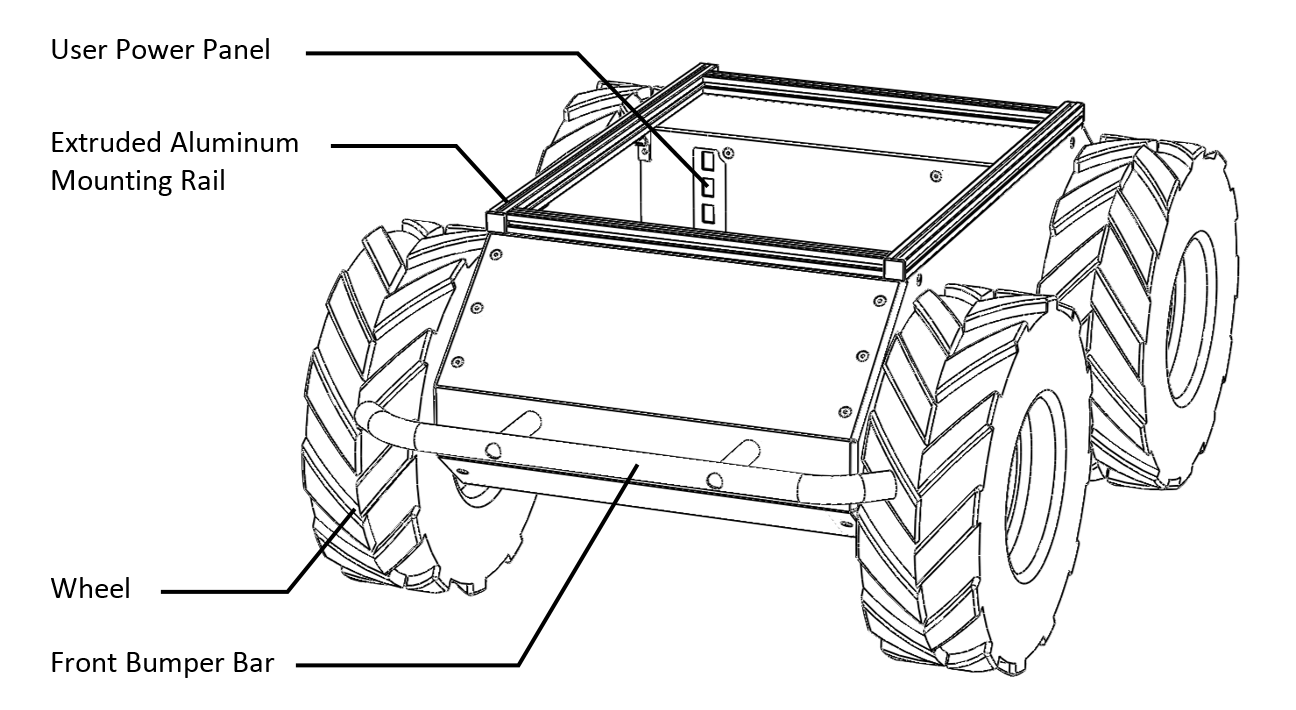
\includegraphics[width=0.9\linewidth]{husky-front.PNG}
  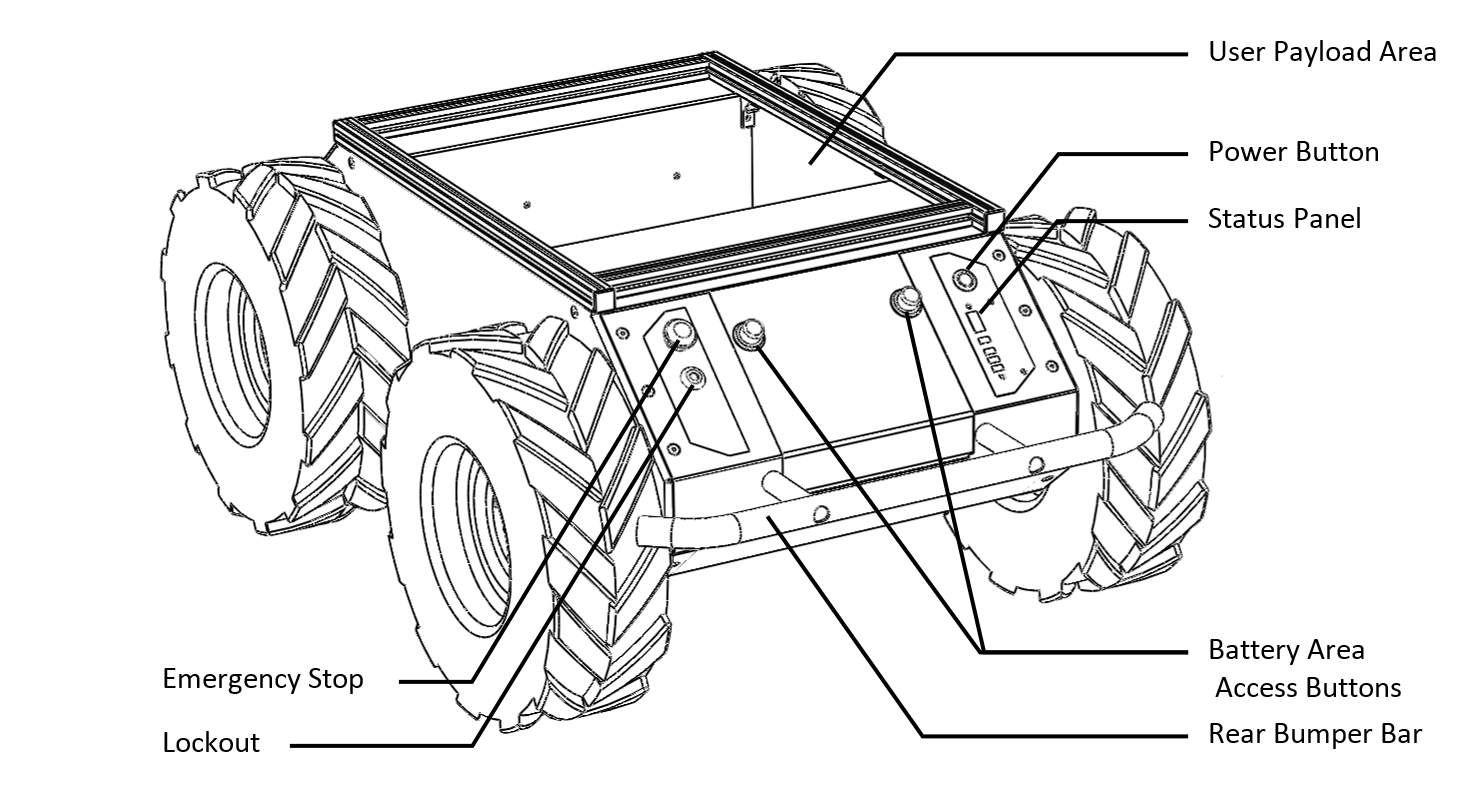
\includegraphics[width=0.9\linewidth]{husky-rear.PNG}
  \caption{Husky at a Glance}
  \label{husky_glance}
\end{figure}
\newpage

\subsection{Status Panel}

The status panel is a display of LED indicators located on the rear of the chassis which 
provide information about the current status of Husky. The indicators are described in \autoref{status_panel}.

\begin{table}[h]
  \renewcommand{\arraystretch}{1.6}
  \centering
    \begin{tabular}{ >{\centering\arraybackslash}m{.1\linewidth} >{\raggedright\arraybackslash}m{.7\linewidth} }
      \hline
    \rowcolor{lightgrey} Icon & Description
      \\ \hline
    
\includegraphics[width=0.7 cm]{battery-mini.png} &
      \textbf{Battery status} The four LED segments provide an approximate indication of the relative lifetime remaining in the battery,
      \\[4pt] \hline
    
\includegraphics[width=0.7 cm]{comm-mini.png} &
      \textbf{Communication status} When green, Husky is receiving a stream of correctly-formatted motion commands, and is ready to drive. When yellow, Husky is receiving commands, but will not drive due to emergency stop or another error. When red, serial communications are currently timed-out.
      \\[4pt] \hline
    
\includegraphics[width=0.7 cm]{err-mini.png} &
      \textbf{General error status} Illuminates red when Husky will not drive due to an error state. Such states include emergency stop, insufficient battery power, or an unspecified software error.
      \\[4pt] \hline
    
\includegraphics[width=0.7 cm]{estop-mini.png} &
      \textbf{Emergency stop status} Illuminates red when Husky will not drive due to the emergency stop being activated, either onboard or wireless (if available).
      \\[4pt] \hline
    
\includegraphics[width=0.7 cm]{charge-mini.png} &
      \textbf{Charge Indicator} Illuminates red when Husky user power is being supplied externally.
      \\[4pt] \hline
    \end{tabular}
  \caption{Husky Status Panel Icons}
  \label{status_panel}
\end{table}
\newpage

\subsection{Orientation References}

The reference frame used by all Clearpath Robotics ground vehicles is based on ISO 8855, and is shown in \autoref{rframe}. Husky is displayed from the front. When commanded with a positive translational velocity (forward), wheels travel in the positive x-direction.
The direction of the axes differs from those used for roll, pitch, and yaw in aircraft, and care should be taken to ensure that data is interpreted correctly.

 \begin{figure}[h]
	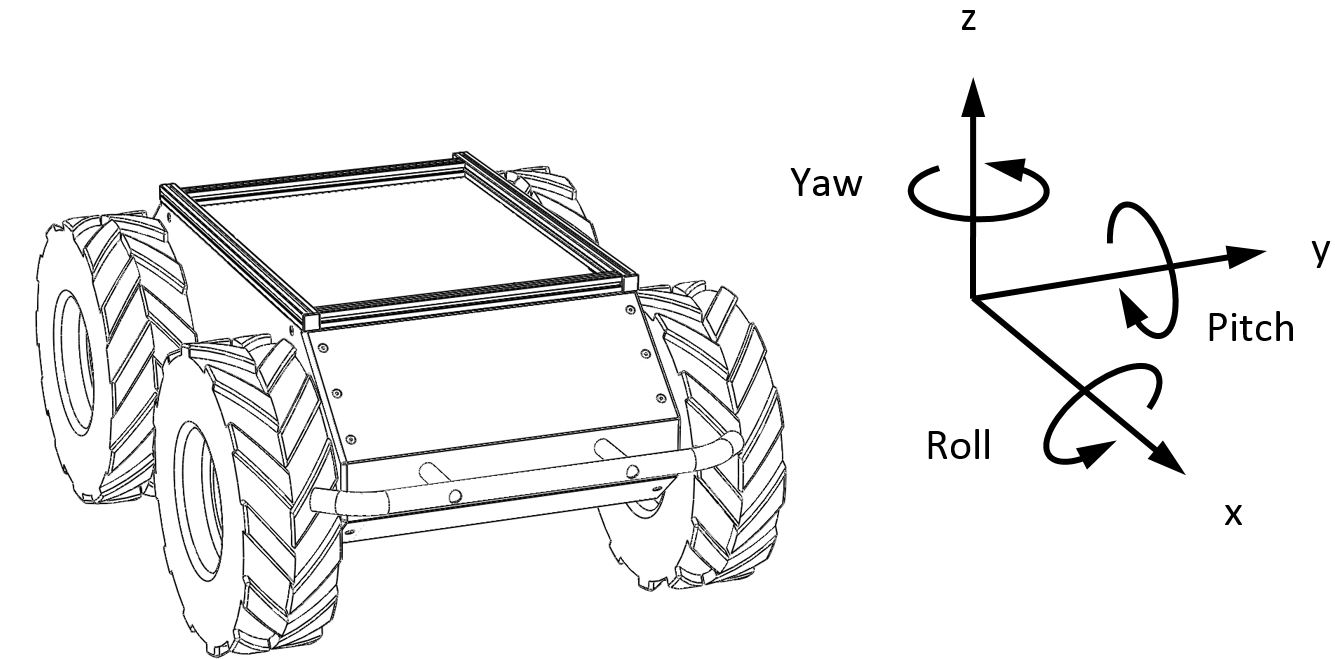
\includegraphics[width=\textwidth]{rframe.png}
	\caption{Husky Reference Frame}
	\label{rframe}
 \end{figure}

\subsection{Pinout Refrences}

Husky provides a female DE-9 connector for communication with a host device. The pinout of this connector is shown in \autoref{pinouttable} .


\begin{figure}[h]
	\centering
	\begin{tabular}{  >{\centering\arraybackslash}m{.4\linewidth} c c c c }
	\multirow{5}{*}{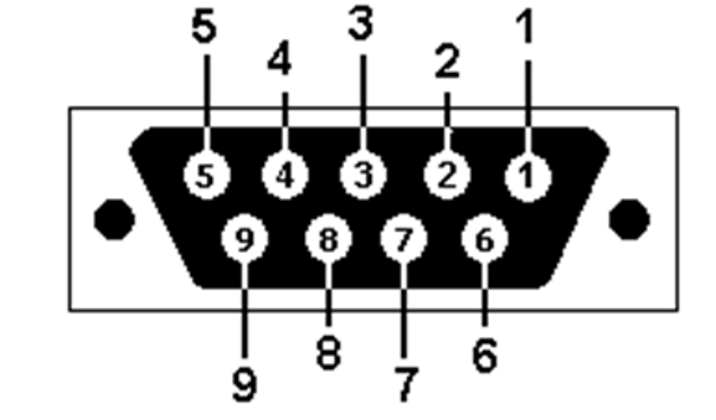
\includegraphics[width=0.4\textwidth]{pinout.png}} \\  \cline{2-5} 
	& \cellcolor{lightgrey}  Pin & \cellcolor{lightgrey}  Name & \cellcolor{lightgrey}  Dir & \cellcolor{lightgrey}  Description \\ \cline{2-5}
	& 2 & RX & IN & Data from Platform\\  \cline{2-5}
	& 3 & TX & OUT & Data to Platform\\ \cline{2-5}
	& 5 & GND & N/A & Common Ground\\ \cline{2-5}
	\end{tabular}
	\newline
	\caption{Husky DE9 Pinout}
	\label{pinouttable}
	
\end{figure}

\newpage
 
\section{System Specifications}

Key specifications of Husky are shown in \autoref{systemspecs} .

\begin{table}[h]
	\centering
	\begin{tabular}{>{\columncolor{lightgrey}}>{\raggedright}m{.25\textwidth} p{.25\textwidth} p{.25\textwidth}} \hline 
	& 990 mm length & 39 in length \\
	& 670 mm width & 26.4 in width \\
	\multirow{-3}{*}{Dimensions} 
	& 390 mm height & 14.6 in height \\ \cline{2-3}
	Track & 555 mm & 21.9 in \\ \hline
	Wheelbase & 512 mm & 20.2 in \\ \hline
	Weight & 50 kg & 110 lbs \\ \hline
	Maximum Payload\footnotemark[1] & 75 kg & 165 lbs \\ \hline
	All-terrain payload\footnotemark[2] & 20 kg & 44 lbs \\ \hline
	Speed (max) & 1.0 m/s & 3.3 ft/s \\ \cline{2-3}
	Ground clearance & 130mm & 5 in \\ \cline{2-3}
	Climb grade & 45\degree & 100\% slope \\ \cline{2-3}
	Traversal grade & 30\degree & 58\% slope \\ \cline{2-3}
	Operating Ambient Temperature & -10 to 30\textsuperscript{o} C & 14 to 86\textsuperscript{o} F \\ \hline 
	& 3 hours typical & \\ 
	\multirow{-2}{*}{Operating time} 
	&\multicolumn{2}{p{.5\textwidth}}{8 hours standby (no motion)}\\ \cline{2-3}
	& 24V 20Ah &\\ 
	\multirow{-2}{*}{Battery}
	& Sealed Lead Acid & \\ \cline{2-3}
	\multirow{2}{*}{Battery charger} & \multicolumn{2}{p{.5\textwidth}}{Short-circuit, over-current, over-voltage and reverse voltage protection}\\ \hline 
	Charge time & 10 hours & \\ \hline
	& 5V / 12V / 24V & \\
	\multirow{-2}{*}{User Power}
	& Each fused at 5A & \\ \hline
	& RS-232 & \\
	\multirow{-2}{*}{Communication}
	& 115200 Baud & \\ \hline
	Wheel Encoders & 78,000 ticks/m & \\ \hline
	& Battery Status & \\
	& Wheel odometry & \\
	\multirow{-3}{*}{Internal Sensing}
	& Motor currents & \\ \hline
	
	\end{tabular}
\newline
\caption{Husky System Specifications}
\label{systemspecs}
\end{table}

\footnotetext[1]{Continuous operation on relatively flat terrain with wide turns}
\footnotetext[2]{Vehicle climbing 30° grade with high-mounted payload, or turning in place in high-friction conditions}
\newpage
\subsection{Vehicle Equations}

As a starting point, Clearpath Robotics recommends using the following relationship between wheel velocity and platform velocity:
\begin{figure}[h]
\centering
$v=\frac{v_r+v_l}{2} , \omega=\frac{v_r-v_l}{w}$
\end{figure}

$v$ represents the instantaneous translational speed of the platform and $w$ the instantaneous rotational speed. $v_r$ and $v_l$ are
the right and left wheel velocities, respectively. $w$ is the effective track of the vehicle, 0.555 m.

\section{Safety}
Clearpath Robotics is committed to high standards of safety. Husky contains several features to protect the safety of users and the integrity of the vehicle.

\subsection{General Warnings}

Husky is a rugged and high-performance vehicle. For the safety of yourself and others, 
always conduct initial experiments and software development with the vehicle raised off the ground. 
Place a wooden crate, a set of sawhorses, a sturdy storage tub, or any other solid flat structure having a 
height greater than 6 inches under Husky to keep the wheels clear of the ground (“up on blocks”).

When starting out, favor slower wheel speeds. Husky’s control loops can accurately maintain velocities 
as low as 0.1 m/s. Operating at such speeds will give you more time to react if things don’t go quite as you expect.

When Husky is operating, keep clear of the wheels, paying particular attention to the pinch hazard which exists between each wheel and the end of the corresponding bumper bar.

\subsection{E-Stop and Lockout}

The red emergency stop button (e-stop) and lockout are located on the back of Husky, opposite the status panel, 
shown in \autoref{estop-lockout}. Power supply to Husky’s motor drivers is enabled by a normally-open relay, 
which is closed in series with the e-stop switch. When in e-stop mode, the status panel e-stop light will illuminate red, 
and Husky will not drive. The commands received during e-stop are not buffered; Husky will always act on the latest commands 
received. This means that if the commands are stopped before the e-stop is released, the Husky will not move. If the 
commands are continued, Husky will move at the speed commanded once the e-stop is released.

\begin{figure}[h]
	\centering
	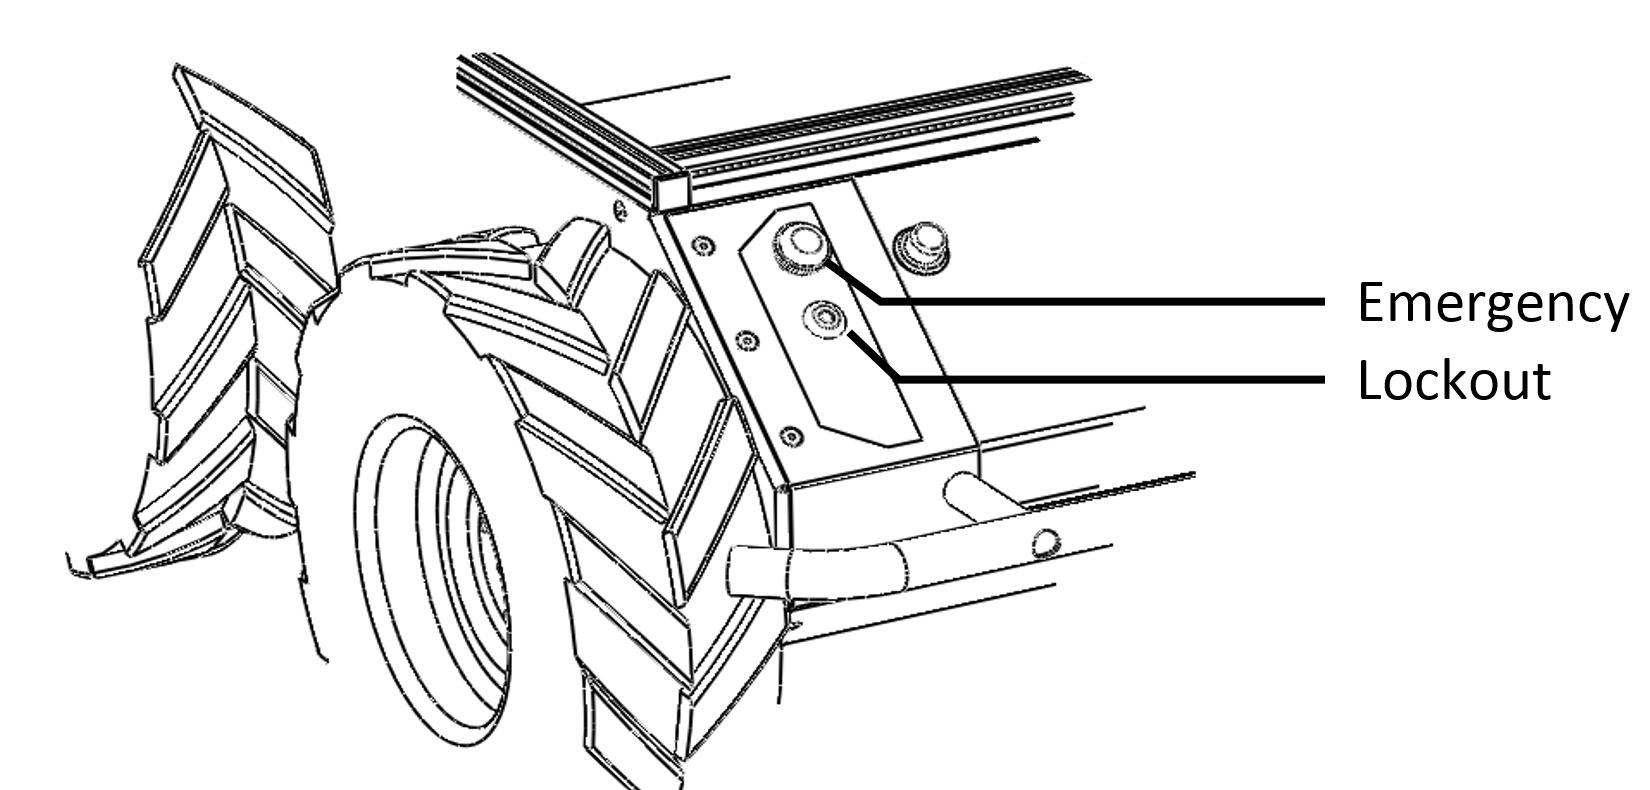
\includegraphics[width=0.6\textwidth]{estop-lockout.png}
	\caption{Husky Emergency Stop and Lockout}
	\label{estop-lockout}
\end{figure}

Always ensure the e-stop button is accessible at all times. Avoid mounting payloads that extend over the rear of Husky and would occlude the e-stop.

The lockout provides a way to secure Husky from performing any type of motion. When in lockout mode, the robot will still power on, but the motors will not drive.

\subsection{Electrical System}
Husky is powered by a single 24V sealed lead-acid battery, similar to the type found in electric wheelchairs, golf carts, 
and other devices. Husky’s battery is capable of delivering 1800W—similar to wall mains. This gives Husky’s motors their 
great performance, however, it is also enough power to cause severe bodily harm. Please observe the following precautions:

\begin{itemize}
	\item Do not tamper with the plug attached to the battery.
	\item Do not tamper with the fuse panel, except to check and change the fuses, and to connect and disconnect the battery plug.
	\item Do not operate Husky without the battery door in place. The battery is not restrained without the door, and will come loose, damaging the fuse panel.
	\item Charge the battery only with the charger provided by Clearpath Robotics.
	\item Please dispose of the batteries properly.
\end{itemize}
	
\subsection{Lifting and transport}
For the safety of users and to maximize the lifetime of Husky, please observe the following when manually transporting the robot:

\begin{itemize}
		\item Husky should be lifted by two persons, firmly gripping the front and rear bumper-bars. 
		The battery can be removed to lighten the load of a manual transport.
		\item Ensure that Husky is e-stopped when transporting short distances and powered off when transporting 
		longer distances.
		\item Note: It is not advised to push Husky, as this can cause damage to the motors
\end{itemize}
\newpage
	
\subsection{Performance Recommendations}

Included in Husky are native software checks and limits to protect the vehicle. However, 
it is recommended to monitor the system’s status during usage with the \lstinline{/status} and \lstinline{/diagnostics} topics. 
These topics provides useful information regarding voltages, currents, temperatures and general health of the system.

The total current draw does not include the motors drivers; it is the current consumed by the MCU and user power ports. 
Husky’s motors are rated to draw 8A continuous, but they will spike to several times this, particularly when traversing 
rough terrain and when turning on the spot. To reduce current draw, consider commanding wider-radius turns from 
your control software.

The temperature is measured in the motor drivers and on the motor casings; the coils inside the motor casings cannot be measured.
Therefore, it is important to note that the temperature measured on the motor casings is a lagging indicator of 
the temperature of the coils inside the casing. Be aware of the delay in heat propagation on the motors during heavy use. 
The thermal limit of the system is 50 C\degree, and the system will shut down if this limit is reached.
Monitoring these fields over longer periods of operation will allow you to ensure that you are not putting 
excessive wear on Husky's motors.
\newpage

\section{Getting Started}

You are ready to go! This section details how to get Husky into action.
To begin, place Husky “up on blocks” as described in the Safety section – make sure the wheels are clear of the ground.

For most Husky setups, there will be an Onboard PC which is directly connected to the Husky and a Remote PC which is used to control Husky and gather data. These two PCs must be set up to communicate with each other.


\subsection{Onboard PC Setup}

If you purchased an Onboard PC from Clearpath Robotics with Husky, it is already installed, connected, and powered. 
Provided on this machine is the officially-supported ROS software for Husky, joystick teleoperation, and any sensor payloads purchased.

If not, or to set up your own Onboard PC, please visit \url{http://wiki.ros.org/Robots/Husky}


\subsection{Connecting the Onboard PC}

Husky’s serial port is located in the user power panel accessible from the user area, shown in \autoref{RS232}.

\begin{figure}[h]
	\centering
	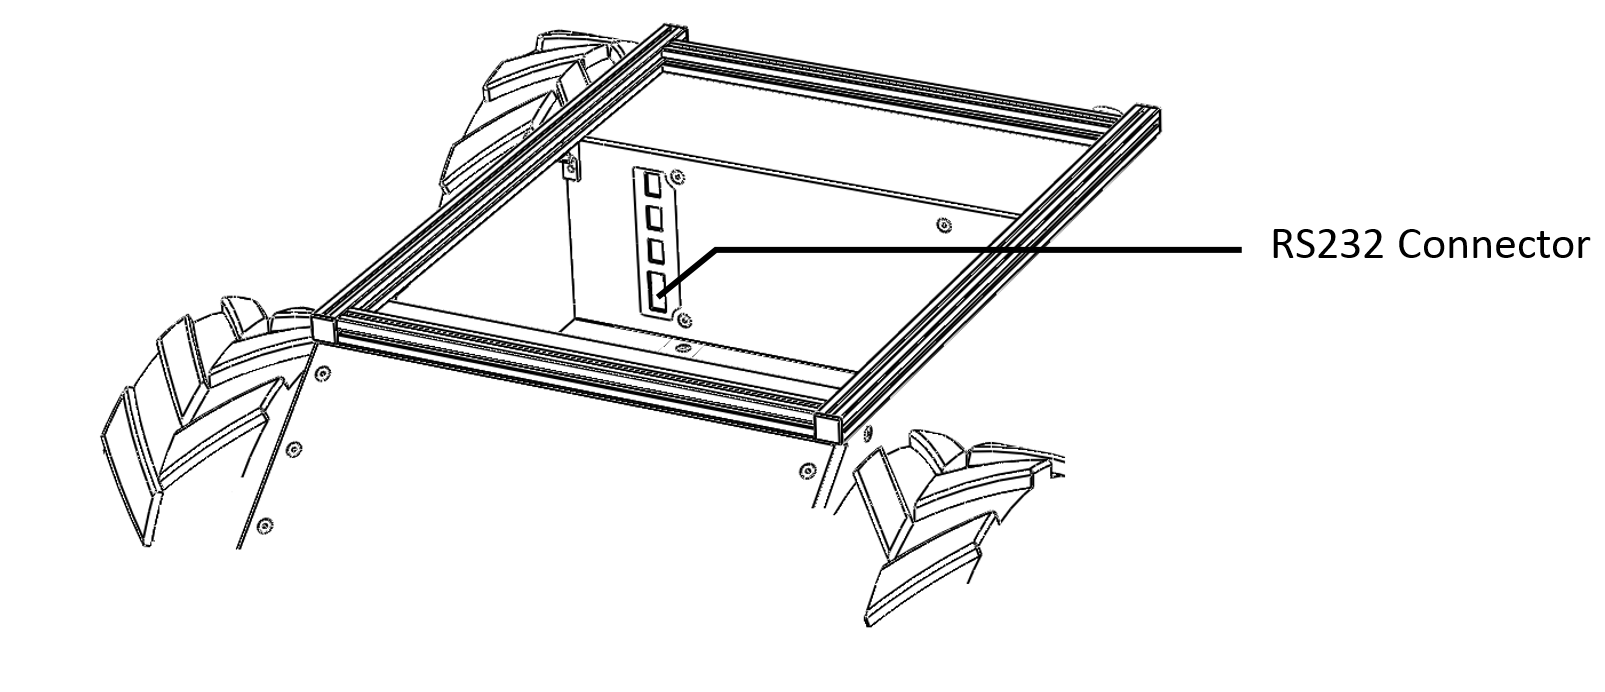
\includegraphics[width=0.8\textwidth]{RS232.png}
	\caption{Husky RS232 Connector}
	\label{RS232}
\end{figure}

The connector is a female DE9, suitable for connection directly to a USB-serial adaptor, 
or to a PC serial port via a straight-through modem cable (not a null modem cable). 
How you connect the Onboard PC to Husky depends on whether the Onboard PC has a dedicated serial port.

\subsection{Remote PC}

Once you have an Onboard PC connected to your Husky with ROS installed, it is recommended to set up your Remote PC.  
Begin by either plugging the Remote PC directly into Husky’s router, or connecting to the same wireless network 
that your Husky was configured to connect to.  

It is now possible to communicate with Husky by either setting up a ROS master environment, or using SSH. SSH is very useful for directly accessing the Onboard PC and to perform software updates.

To access the Onboard PC, you can SSH into Husky:

\begin{lstlisting} 
ssh administrator@<IP_OF_ONBOARD_PC>
\end{lstlisting}

However, some features are not available through SSH and so it is recommended to set up a ROS master environment. 
If you are using an Onboard PC supplied by Clearapth, or using the Clearpath ISO on your own Onboard PC, Husky will
already be configured as the ROS master.

On your Remote PC you will want to add the Onboard PC hostname to your \lstinline{/etc/hosts} file along with it's IP address 
so your Remote PC can communicate with Husky via it's hostname.

Husky's hostname (Onboard PC) will either be set by Clearpath, or defined by the user during the 
installation process, in any case, you can verify the hostname and IP address of Husky using
the following commands during an SSH session with the Onboard  PC.

\begin{lstlisting}
hostname
hostname -i
\end{lstlisting}


Once Husky's hostname and IP address have been added to \lstinline{/etc/hosts}, ensure the Remote PC
can communicate with Husky via hostname:

\begin{lstlisting}
ping HUSKY'S HOSTNAME
\end{lstlisting}

If both computers can ping each other, then set the following ROS environment variable on your remote PC.

\begin{lstlisting}
export ROS_MASTER_URI=http://<HUSKY'S HOSTNAME>:11311
export ROS_HOSTNAME=<REMOTE PC'S HOSTNAME>
\end{lstlisting}

You can then verify your connection by using:

\begin{lstlisting}
rostopic list
rostopic echo /tf
\end{lstlisting}

If your Husky is equipped with an external radio or base station that is connected to a subnet different than your Remote PC, 
you will have to set up a static route to communicate with Husky. You can find the IP address of Husky’s 
router using the routers built in interface or a third party application.
\begin{lstlisting} 
sudo route add -net <IP OF HUSKY> netmask 255.255.255.255 gw <ADDRESS OF EXTERNAL RADIO>
\end{lstlisting}

\newpage

\subsection{Connecting Power}
Husky comes with the battery fully charged and installed, but disconnected for safety during shipping. 
To reconnect the battery:

\begin{enumerate}
	\item Ensure Husky’s main power button is in the outer “off” position and the e-stop is activated.
	\item Using curled index fingers to grip the battery door latches, press with thumbs on the latch buttons and lift the battery door free of the chassis.
	\item Carefully connect the battery plug to the mating connector in the fuse panel, shown in \autoref{battery-area}. Ensure that it is firmly seated and clicks into place. It will be difficult to connect it in the incorrect polarity.
	\item Replace the battery door cover, ensuring that it clicks into place and is flush with the rear panel.
\end{enumerate}

\begin{figure}[h]
	\centering
	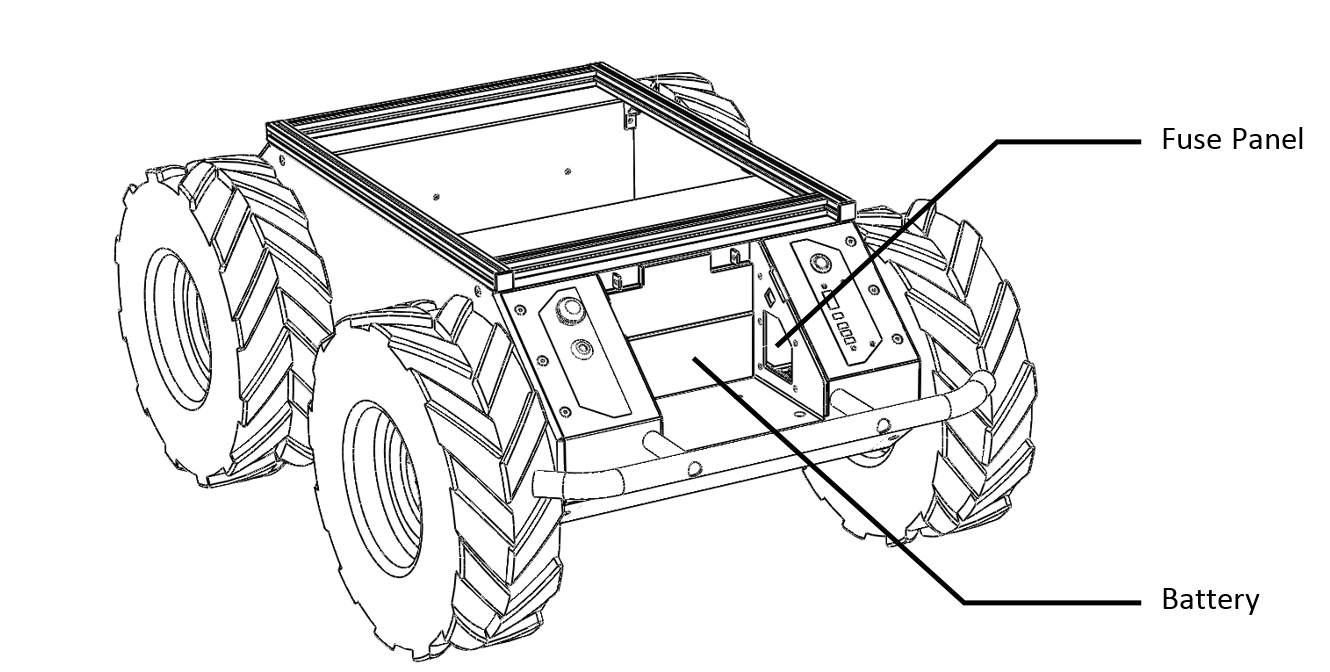
\includegraphics[width=0.8\textwidth]{battery-area.png}
	\caption{Husky Battery Area}
	\label{battery-area}
\end{figure}

To power on Husky, firmly press the power button located above the status panel. It will illuminate blue, and the 
status panel lights will show a brief test pattern. The comm status light will turn red, as the PC is not yet 
communicating with Husky.

The stop status light will be red if the e-stop is pressed. If it is not, press the e-stop button and 
verify that the stop light illuminates. Leave the platform in an e-stop state until it is successfully receiving commands.

\subsection{User Bay Power Connections}
The user area power terminals are capable of supplying 5V, 12V, and 24V at up to 5A each for powering Husky’s payloads.  
Each terminal comes equipped with a removable connector into which your payload power leads may connect.

To begin, expose about 5mm of bare wire from the payload power leads. The power connector features two 
openings on the top for each pin; a square hole and a round hole. Insert a 2mm wide flat head screwdriver 
into the square hole to “open” the adjacent round hole as seen in \autoref{connectors}. Slide the power lead into the round hole, and then 
remove the screwdriver to lock the wire in place.

\begin{figure}[h]
	\centering
	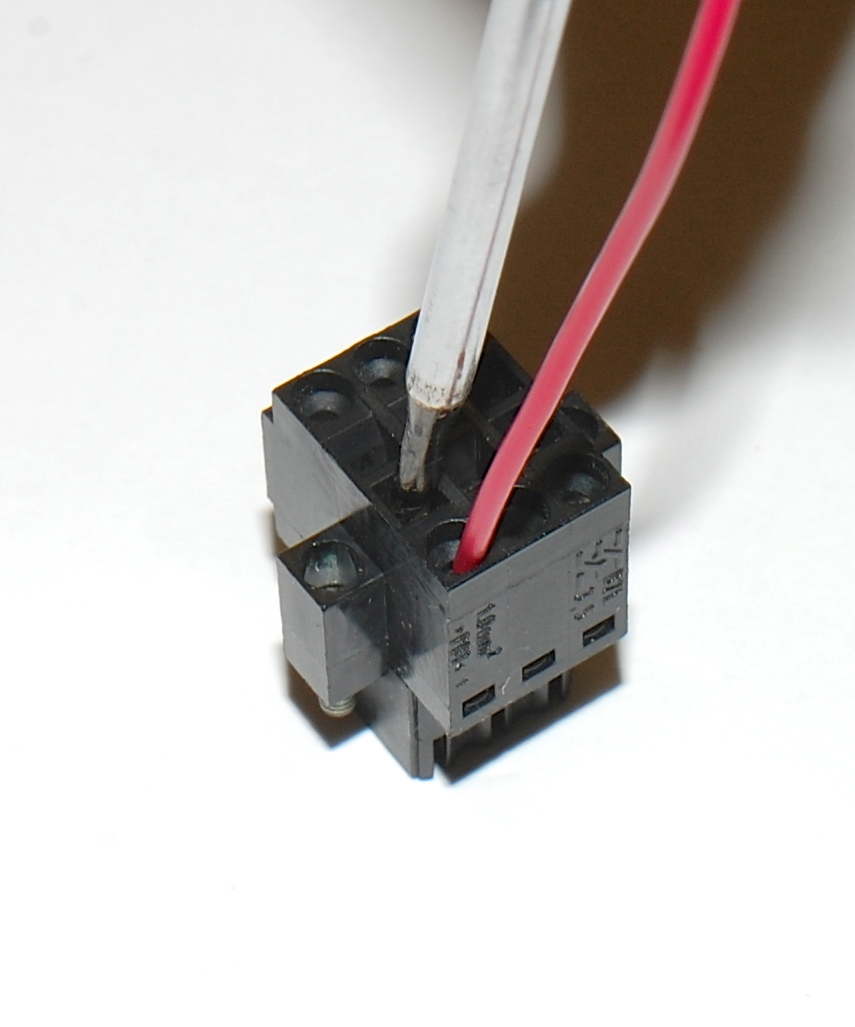
\includegraphics[width=0.3\textwidth]{power-connector-1.png}
	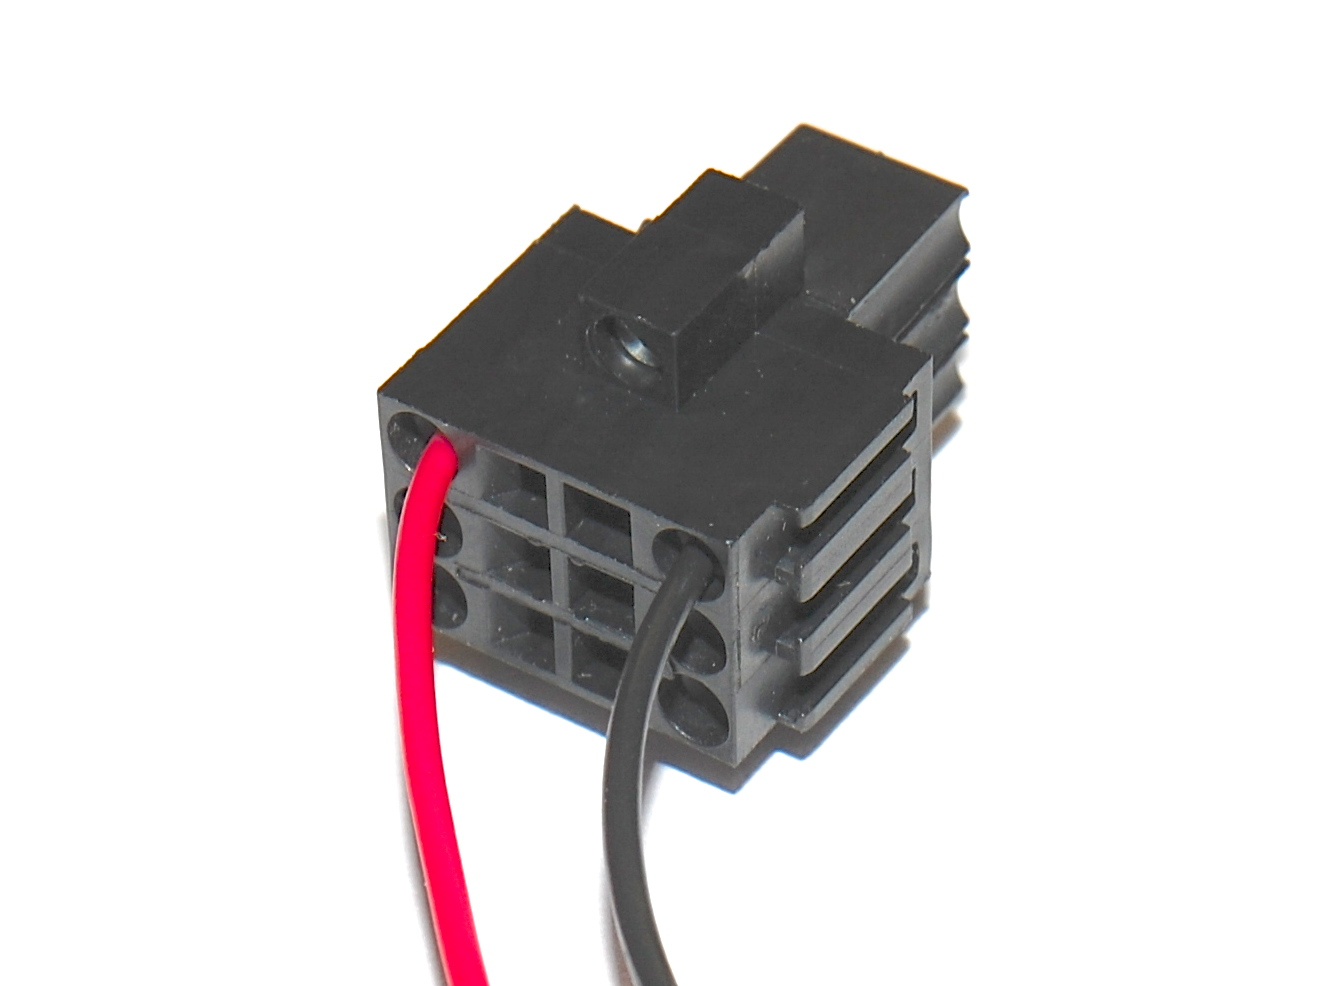
\includegraphics[width=0.5\textwidth]{power-connector-2.png}
	\caption{Removable Power Connectors}
	\label{connectors}
\end{figure}

When connecting payloads, be sure to observe correct polarity as marked on the inside of the user bay. 
Do not exceed the 5A maximum current limit of each power rail; failure to do so may result in damage 
to Husky or your payload.

For more technical information on the power connectors, as well as their corresponding mating connectors, please visit: \url{http://www.digikey.com/product-search/en?vendor=0&keywords=281-1856-ND&cur=USD}

\subsection{Verification}
If a computer was purchased with Husky, it will be setup to interface automatically upon startup. 
60-90 seconds after booting up, the Husky comms light will change from red to green 
(or yellow, depending on e-stop status), indicating that ROS is up and has established communications with Husky.

To tele-operate Husky, plug a USB joystick into the included Onboard PC, and release the emergency stop. 
After a few seconds, ROS should recognize the joystick and begin passing commands through to the mobile platform. 
Press the enable button (typically button 1), and use the main joystick axis or left thumbstick to drive Husky.

Direct control using the Python or C++ interfaces is also possible, the API is available at
\url{http://www.clearpathrobotics.com/husky/downloads} However, please note that Clearpath Robotics no 
longer provides support for these packages, and are they supplied "as is".

\section{Using ROS}
Robot Operating System (ROS) is an extensible framework for controlling and working with robotic systems. 
Clearpath Robotics recommends using ROS with Husky. If this is your first time using ROS, it is strongly 
recommended to run through our series of ROS101 tutorials to learn the basics of ROS 
\url{http://support.clearpathrobotics.com}. If you did not purchase a PC from Clearpath Robotics, please visit \url{http://wiki.ros.org/Robots/Husky} 
to set up your own Onboard PC.

\subsection{Nodes}
You can use \lstinline{rosnode list} to see all the nodes running by default on a Husky computer. 
The baseline set of these is presented with commentary in \autoref{nodes-table}.

\bgroup
\begin{table}[h]
	\centering
	\begin{tabular}{>{\columncolor{lightgrey}}m{.25\linewidth} m{.5\linewidth}} \hline
	Node & Description \\ \hline
	/husky\_node & Provides control and communication between the Husky platform and ROS. Accepts velocity commands and provides system feedback on /status \\ \hline
	/robot\_state\_publisher & Subscribes to /joint\_states and publishes the robot's state to tf \\ \hline
	/bluetooth\_teleop & Publishes velocity commands from a joystick to /twist\_mux \\ \hline
	/twist\_mux & Takes in multiple sources of velocity commands, and prioritizes what actually gets sent to the controller \\ \hline
	/ekf\_localization & Part of the robot localization package, more information regarding this package can be found at \url{http://wiki.ros.org/robot_localization } \\ \hline 
	\end{tabular}
	\caption{Standard Husky Nodes}	
	\label{nodes-table}
\end{table}
\egroup
\newpage
\subsection{Topics}
You can view all topics that are active using \lstinline{rostopc list}. Some of the base topics are listed in \autoref{topics-table} and \autoref{topics-motion}.

\begin{table}[h]
	\centering
	\begin{tabular}{>{\columncolor{lightgrey}}m{.3\linewidth} m{.25\linewidth} m{.3\linewidth}} \hline
		Topic & Message type & Description\\ \hline
<<<<<<< HEAD
		\lstinline|/bluetooth_teleop/joy| & \lstinline|sensor_msgs/Joy| & Receives joystick commands, echo this topic to verify your controller is publishing  \\ \hline
		\lstinline|/tf| & \lstinline|tf2_msgs/TFMessage| & Transforms between coordinate frames, this should always be publishing, and hence a good topic to echo to test your ROS connection \\ \hline
		\lstinline|/status| & \lstinline|husky_msgs/HuskyStatus| & Displays system status information\\ \hline
		\lstinline|/estop| & \lstinline|std_msgs/Bool| & Displays the estop status\\ \hline
		\lstinline|/odometry/filtered| & \lstinline|nav_msgs/Odometry| &  The odometry estimate of the robot from \lstinline|/ekf_localization|\\ \hline
=======
		\lstinline!bluetooth_teleop/joy! & \lstinline!sensor_msgs/Joy! & Receives joystick commands, echo this topic to verify your controller is publishing \\ \hline
		\lstinline!/tf! & \lstinline!tf2_msgs/TFMessage! & Transforms between coordinate frames, this should always be publishing, and hence a good topic to echo to test your ROS connection \\ \hline
		\lstinline!/status! & \lstinline!husky_msgs/HuskyStatus! & Displays system status information\\ \hline
		\lstinline!/estop! & \lstinline!std_msgs/Bool! & Displays the estop status\\ \hline
		\lstinline!/odometry/filtered! & \lstinline!nav_msgs/Odometry! &  The odometry estimate of the robot from \lstinline!/ekf_localization!\\ \hline
>>>>>>> 46e23147c6a4b9b20978f874f25644e6b309b5b3
	\end{tabular}
	\caption{Standard Husky Topics}
	\label{topics-table}
\end{table}

\begin{table}[h]
	\centering
	\begin{tabular}{>{\columncolor{lightgrey}}m{.3\linewidth} m{.25\linewidth} m{.3\linewidth}} \hline
<<<<<<< HEAD
		Motion Topics & \lstinline|twist_mux| Priority & Description\\ \hline
		\lstinline|husky_velocity_controller/cmd_vel| & - & Receives motion commands from \lstinline|twist_mux| based off their priority\\ \hline
		\lstinline|joy_teleop/cmd_vel| & 10 & Joystick teleop input\\ \hline
		\lstinline|twist_marker_server/cmd_vel| & 8 & Interactive marker teleop input\\ \hline
		\lstinline|move_base/cmd_vel| & 2 & Autonomous movement input, for the husky navigation packages\\ \hline
		\lstinline|cmd_vel| & 1 & Miscellaneous external input \\ \hline
=======
		Motion Topics & \lstinline!twist_mux! Priority & Description\\ \hline
		\lstinline!husky_velocity_controller/cmd_vel! & - & Receives motion commands from \lstinline!twist_mux! based off their priority\\ \hline
		\lstinline!joy_teleop/cmd_vel! & 10 & Joystick teleop input\\ \hline
		\lstinline!twist_marker_server/cmd_vel! & 8 & Interactive marker teleop input\\ \hline
		\lstinline!move_base/cmd_vel! & 2 & Autonomous movement input, for the husky navigation packages\\ \hline
		\lstinline!cmd_vel! & 1 & Miscellaneous external input \\ \hline
>>>>>>> 46e23147c6a4b9b20978f874f25644e6b309b5b3
	\end{tabular}
	\caption{Standard Husky Motion Topics}
	\label{topics-motion}
\end{table}

\subsection{Workspace}
The expected model for extending Husky is to create a new ROS Workspace in the user’s home directory, 
and add packages there. You can roslaunch additional nodes against the ROS Master already running on Husky 
without needing to stop or start anything else. See the Overlays page on the ROS wiki for more details: 
\url{http://wiki.ros.org/catkin/Tutorials/workspace_overlaying}
 
When it comes time for some of your own code to be launched on startup of Husky, edit the default workspace setup file, 
located in \lstinline{/etc/ros/setup.bash}. Change the final line from the default to instead source your own workspace. 
When this is done, copy the launch file for your software into the \lstinline{robot_upstart} folder, which is located at 
\lstinline{/etc/ros/hydro/husky-core.d}. Now restart the Husky background service and your nodes should come 
up with the rest of Husky:

\begin{lstlisting}
sudo service husky-core restart
\end{lstlisting}

For more details on this process, please see the ROS wiki page about upstart, located at: \url{http://wiki.ros.org/robot_upstart} 

\subsection{Payloads}
You can find a list of supported packages and related documentation for payloads on Clearpath Robotics’ 
ROS Wiki page here: \url{http://wiki.ros.org/ClearpathRobotics}
\newpage

\section{Battery and Maintenance}
Husky A200 is built for rugged, long-term use. Here are some steps that can be 
taken to maintain and extend the life of the platform even further.

\subsection{Charging}
The battery shipped with Husky A200 may be charged off-board, or while still inside of Husky. 
If charging while installed, you will need to open the access door to the battery area, and 
disconnect the battery from its connector in the fuse panel. From there:

\begin{enumerate}
	\item Connect the DC output cable from the charger to the battery terminal connector.
	\item Plug the charger power cord into the charger and then into a wall receptacle.
	\item The POWER LED and CHARGING LED lights on the charger will illuminate.
	\item When battery is fully charged, the CHARGING LED light will turn off. 
	\item Unplug the charger from the wall, and then disconnect it from the battery.
\end{enumerate}

The battery charger shipped with Clearpath Robotics’ lead-acid 
battery-powered products uses a three-state charge cycle.

\begin{enumerate}
		\item A fast, high current initial charge, until the battery voltage reaches 29.6V.
		\item A topping charge, during which the battery charges at 29.6V constant voltage 
		until the current decreases to 500 mA.
		\item A precision float charge, during which the battery voltage is held at 27.6V. 
		This mode allows the charger to remain connected to the battery during periods of non-use, 
		keeping it in a state of full charge. When in this mode, the CHARGING LED will be off.
\end{enumerate}		

\subsection{Battery Care}
Husky’s power supply is a sealed 24 V lead acid battery pack (VRLA), providing 20 ampere-hours of charge. These tips are 
intended to help keep your Husky Lead-Acid Battery in tip-top shape.  With proper maintenance, the battery should 
maintain the majority of its capacity for hundreds of cycles.

The most damaging thing to a lead-acid battery is a phenomenon called sulfation.  
When a lead-acid battery is left in an uncharged state for long periods of time, 
sulfate crystals solidify on the electrodes of the battery.  This effect can be permanent, 
and it causes premature reduction in capacity.  Therefore, it is important to fully charge 
the battery as soon as you are finished using it, regardless of how much capacity remains

Your Husky ships with a three-stage battery charger that completely charges a Husky battery.  
Charging occurs in three stages: Constant current, topping charge, and float charge.  
The bulk of the capacity (70\%) is regained during the first stage.

It is important to let the charger complete all three stages whenever possible, 
to help maintain the life of the battery.  The initial stage will take 5-7 hours,
and a complete charge may take up to 14 hours.

\begin{figure}[h]
	\centering
	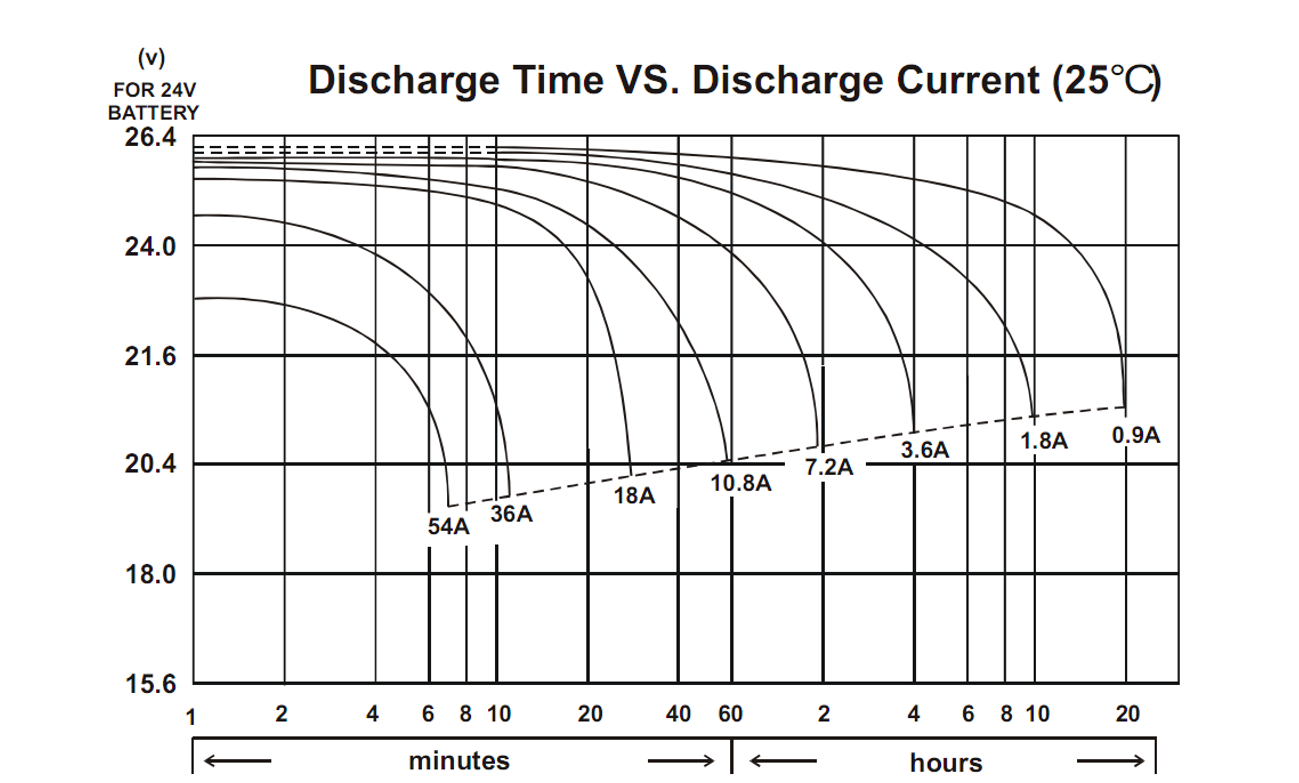
\includegraphics[width=0.7\textwidth]{battery-chart.png}
	\caption{Husky Battery Voltage Characteristics}
	\label{battery-chart}
\end{figure}

In general, following these tips will help maximize the life of the battery:

\begin{itemize}
	\item Always fully charge the battery as soon as you are finished using it.
	\item Charge batteries at room temperature.  Never charge lead-acid batteries at temperatures above 35 degrees Celcius.
	\item Charge batteries in a well-ventilated area.
	\item Do not allow the battery to freeze.  A low battery will freeze sooner than a fully charged one.  Never charge a frozen battery.
	\item Stored batteries should be topped up every month.  Completely cycle batteries every 4-6 months.
	\item At a discharge rate of 50% DOD (depth of discharge), the lifecycle of the Husky battery is 450-550 cycles.  
	After this point, reduced capacity will be apparent.
	\item Regularly discharging the battery below 50% DOD will reduce the lifecycle of the battery, sometimes to less than 300 cycles.
\end{itemize}

\subsection{Wheels}
Tire pressure may change with temperature and should be checked periodically with a pressure gauge. 
Inspecting tires, releasing pressure, and inflating tires are completed through the tire’s inflation stem. 
Tire pressure should not exceed 20psi, and lower pressure may be desired based on terrain requirements.

If a tire must be removed, first unfasten the four M5 Socket Head Cap Screws that join the wheel to the axle hub,
and slide it off the axle. When replacing the tire, screws should be tightened to 3.7 ft-lb [5 N-m] torque.

\subsection{Chassis}
Husky is an all-terrain robot, but it is not waterproof. Care should be taken that no part of the main 
chassis is ever submerged in water. When the chassis becomes wet or dirty, wipe it down with a damp cloth 
and dry with a towel.

If water is suspected to have entered the Husky A200 chassis, remove the battery and allow Husky to fully dry for a minimum of 24 hours.

\section{Tips and Troubleshooting}

\subsection{Mechanical Tips}
Husky’s wheels can handle a range of different terrains, but work best when inflated to the proper pressure. 
Lower tire pressures, for example 10 psi, ensure better traction in rough and varied terrain, where rocks or 
other obstacles may be encountered. This has the adverse effect of lowering drivetrain efficiency and decreasing 
battery charge, so high pressures up to a maximum of 20 psi should be used when driving on flat surfaces. 

\subsection{Troubleshooting}

This section lists a few possible issues which may be encountered:

\begin{itemize}
<<<<<<< HEAD
	\item The blue light around the power button does not display when pressing the power button. Ensure that the battery is charged and correctly connected. Use a multi-meter to verify the voltage on the battery terminals.
	\item Comm light stays red/flickers. Your program may not be sending motion commands faster than 10Hz. If there is a poor quality connection, some commands may be lost, so it may be necessary to increase the frequency of commands sent. The maximum frequency commands can be sent is 50Hz
	\item E-stop light illuminated. Twist the red e-stop to release it, and confirm that the robot is not locked out.
	\item Battery indicator flashing. Battery voltage is too low for Husky to drive the motors. Charge the battery and try again.
	\item A ROS package isn't starting. Verify the upstart logs, \lstinline{/var/log/upstart/husky_core.log} to see if there are any error during upstart.
	\item Husky experiences momentary drops in communication.  It's possible the robot has reached the thermal limit, or current limit. The maximum current limits are set to 18.3A, however, as  the motors are only rated for 8A continuous, anything above that will trigger the current limit eventually, the higher above this limit, the more quickly it will trigger.  If you are unsure whether this is the case, feel free to contact support@clearpathrobotics.com with a rosbag of your system. Clearpath robotics also offers a high torque upgrade if more torque is required for your project.
=======
	\item \textbf{The blue light around the power button does not display when pressing the power button.} Ensure that the battery is charged and correctly connected. Use a multi-meter to verify the voltage on the battery terminals.
	\item \textbf{Comm light stays red/flickers.} Your program may not be sending motion commands faster than 10Hz. If there is a poor quality connection, some commands may be lost, so it may be necessary to increase the frequency of commands sent. The maximum frequency commands can be sent is 50Hz
	\item \textbf{E-stop light illuminated.} Twist the red e-stop to release it, and confirm that the robot is not locked out.
	\item \textbf{Battery indicator flashing.} Battery voltage is too low for Husky to drive the motors. Charge the battery and try again.
	\item \textbf{A ROS package isn't starting.} Verify the upstart logs, \lstinline{/var/log/upstart/husky_core.log} to see if there are any error during upstart.
	\item \textbf{Husky experiences momentary drops in communication.} It's possible the robot has reached the thermal limit, or current limit. The maximum current limits are set to 18.3A, however, as  the motors are only rated for 8A continuous, anything above that will trigger the current limit eventually, the higher above this limit, the more quickly it will trigger.  If you are unsure whether this is the case, feel free to contact support@clearpathrobotics.com with a rosbag of your system. Clearpath robotics also offers a high torque upgrade if more torque is required for your project.
>>>>>>> 46e23147c6a4b9b20978f874f25644e6b309b5b3
\end{itemize}
	
If you experience setup issues that aren’t listed here, or the suggested solution isn’t working out, please get in touch with our support team so we can help: support@clearpathrobotics.com.

\newpage
\section{Product Dimensions}

\begin{figure}[h]
	\centering
	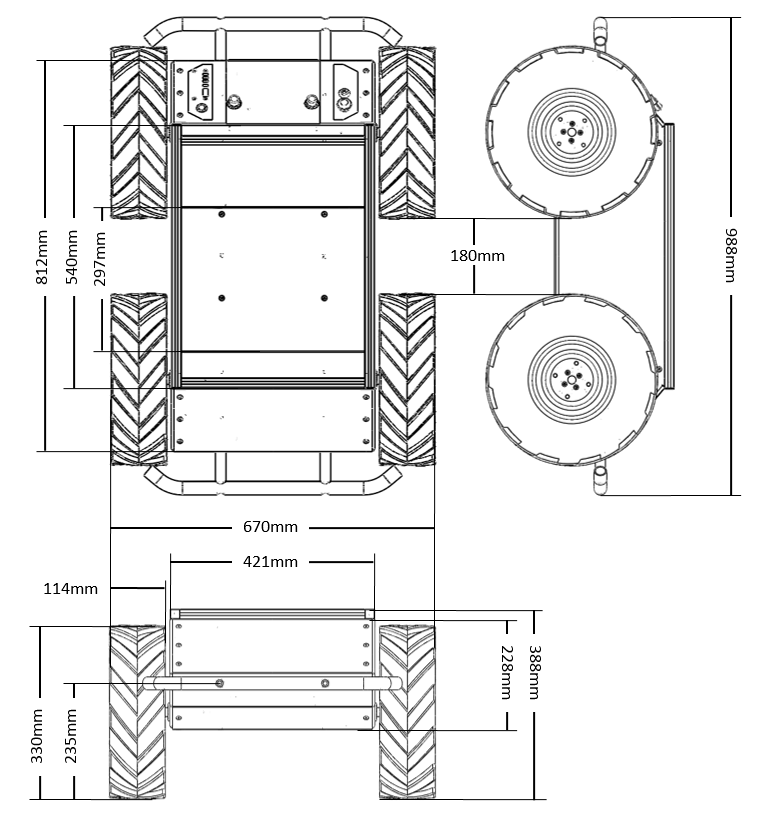
\includegraphics[width=.9\textwidth]{husky-dimensions.png}
	\caption{Husky Dimensions}
\end{figure}
\newpage
\section{Service and Support}
Clearpath is committed to your success with Husky. Please get in touch with us and we'll
do our best to get you rolling again quickly: \href{mailto:support@clearpathrobotics.com}{support@clearpathrobotics.com}
or visit out knowledge base for at \href{http://support.clearpathrobotics.com}{support.clearpathrobotics.com}

To get in touch with our sales team regarding Husky or other Clearpath Robotics products, please
email \href{mailto:sales@clearpathrobotics.com}{sales@clearpathrobotics.com}.

If you have an issue that is specifically about ROS and is something which may be of interest
to the broader community, consider asking it on \href{http://answers.ros.org}{answers.ros.org}.
If you don't get a satisfactory response, please ping us and include a link to your question
as posted there. If appropriate, we'll answer in the ROS Answers context for the benefit of the
community.


\end{document}
